\subsubsection{Analizador de Fourier }
    
    El analizador de fourier, posee un conjunto de filtros donde cada uno de los 
    mismos se encuentran ligeramente desfasados entre si y repartidos de manera 
    uniforme sobre el margen de frecuencia que se desea analizar, tal como se observa
    en la Figura~\ref{fig:EsqInicialFourier}. El conjunto de filtros puede formar 
    parte de un sistema mas complejo, donde sus salidas pueden ser multiplexadas 
    y mostradas en conjunto con un amplificador vertical en una pantalla y a su ves, 
    el multiplexor con un contador, aparte de seleccionar el conjunto de filtros, 
    generar una señal de rampa escalera para posteriormente pasar por un 
    amplificador horizontal y realizar un barrio de eje horizontal de la pantalla 
    para poder visualizar el espectro en frecuencia de una señal. En la 
    Figura~\ref{fig:EsqAnalizadorDeFourierBasico}, se muestra un diagrama en bloques 
    simplificado de un analizador de fourier el cual, su principal 
    ventaja es que, el análisis se hace practicamente en forma simultánea en todo 
    el espectro. Pero dichos instrumentos poseen como desventaja una excesiva 
    complejidad del sistema y a su vez poseen baja resolución con un \textit{spam} 
    (margen de frecuencia de trabajo) fijo.
    \begin{figure}[H]
        \centering
        \begin{subfigure}[H]{0.48\textwidth}
          \frame{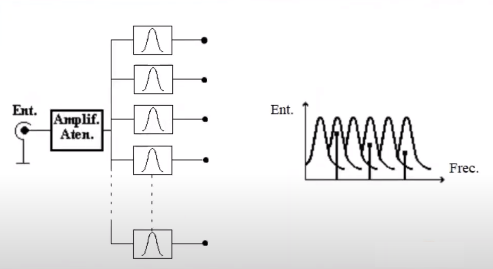
\includegraphics[width=\textwidth]{Imagenes/MarcoTeorico/EsqInicialAnalizDeFourier.png}}
          \caption{Conjunto de Filtros.}
          \label{fig:EsqInicialFourier}
        \end{subfigure}
        \hfill 
        \begin{subfigure}[H]{0.45\textwidth}
          \frame{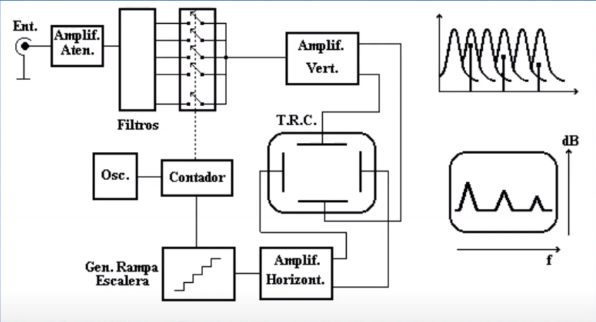
\includegraphics[width=\textwidth]{Imagenes/MarcoTeorico/EsqDeAnalizadorDeFourierBasico.png}}
          \caption{Esq. en bloques simplificador.}
          \label{fig:EsqAnalizadorDeFourierBasico}
        \end{subfigure}
        \caption{Analizar de fourier básico.}
        \label{fig:AnalizadorDeFourier}
      \end{figure}
       